%!TEX root = ../thesis.tex

\section{Cassandra}
\label{sec:theory:cassandra}
Cassandra \cite{CassandraApacheDocs} \cite{CassandraDataStaxDocs} \cite{lakshman2010cassandra} is a high performance, scalable, fault tolerant (i.e. no single point of failure), distributed post-relational database solution, which combines benefits of Google Bigtable \cite{chang2008bigtable} and Amazon Dynamo \cite{decandia2007dynamo}.

\subsection{Key features}
Its key features are:
\begin{itemize}
\item masterless architecture -- there is no distinguished node to coordinate the work, thus no single point of failure,
\item linear scale performance -- data are distributed among nodes, thus in order to handle more data, nodes are added to the cluster (see Section \ref{sec:theory:cassandra:linear}),
\item continuous availability -- data are replicated in the cluster, therefore as long as there are replicas then data are available,
\item flexible data model -- wide-row storage in which each column can have different schema, (described in Section \ref{sec:theory:cassandra:datamodel}),
\item multi data center support -- explicit support and dedicated configuration for multiple data centers,
\item all nodes accept reads and writes -- as consequence of masterless architecture each node in the cluster is able handle any request, 
\item Cassandra Query Language -- language similar in syntax to SQL (see Section \ref{sec:theory:cassandra:cql}).
\end{itemize}

\subsection{Architecture}
Cassandra has a masterless \emph{ring} architecture, in which all nodes are equally significant, and there is no master node, therefore there is no single point of failure (SPOF). Cassandra uses replication and provides continous availability, due to redundancy of both data and node functions.
Inter-node communication bases on scalable and distributed \emph{Gossip} protocol.

A cluster presented on Figure \ref{fig:archCluster} consists of 2 data centers: DC1 and DC2, where DC1 is represented by blue nodes and DC2 by red nodes. All nodes within the cluster use peer to peer communication. Nodes with dashed border are replica nodes of a key $k$. Note that, replicas exist in both data centers, therefore if first data center fails, then $k$ is still accessible from second data center.

\begin{figure}[H]
\centering
\begin{tikzpicture}[->,>=stealth',shorten >=1pt,auto,node distance=3.5cm,
  thick,main node 1/.style={circle,fill=blue!20,draw,
  ,minimum size=5mm},
  main node 1/.style={circle,fill=blue!20,draw,
  ,minimum size=5mm},
  main node 2/.style={circle,fill=blue!20,draw,
  ,minimum size=5mm},
  main node 3/.style={circle,dashed,fill=blue!20,draw,
  ,minimum size=5mm},
  main node 4/.style={circle,fill=red!20,draw,
  ,minimum size=5mm},
  main node 5/.style={circle,dashed,fill=red!20,draw,
  ,minimum size=5mm},
  main node 6/.style={circle,dashed,fill=red!20,draw,
  ,minimum size=5mm}]

\node[draw, text width=3cm] at (-6,3.5) {a key k is replicated on dashed nodes, RF=3};

\draw[thick, line width=3mm, gray, opacity=0.3] (0,0) circle (4cm);

\foreach \a in {1,2,...,6}{
\draw (\a*360/6: 4cm) node[main node \a] (\a) {Node \a};
}

\foreach \x in {1,...,6}
    \foreach \y [count=\yi] in {1,...,6}  
      \draw (\x)--(\yi) ;


\end{tikzpicture}
\caption{A cluster on the token ring}
\label{fig:archCluster}
\end{figure}

\subsubsection{Token ring}
Cassandra's cluster consists of nodes placed on the token ring. Figure \ref{fig:replicationRing} presents cluster with \N{4}, where each node is associated with \emph{token range}, which is part of the token ring. 

Partitioning in Cassandra is implemented by assigning tokens, which are numbers computed by a some function (usually hash function), to keys and storing data in a node for which token is in its token range. 

\subsection{Replication}
Cassandra supports configurable \emph{replication factor} (see Definition \ref{def:replicationFactor}) defined per \emph{keyspace} (Section \ref{sec:theory:cassandra:datamodel}). Figure \ref{fig:replicationRing} shows a replication of the token $91$ in the cluster with $4$ nodes and the token ring with tokens ranging from $0$ to $99$. 
Each node is the \emph{primary replica} for the token range placed counter clock-wise to it, thus node $1$ is the primary replica for range $75-0$, node $2$ for $51-75$, node $3$ for $26-50$, and node $4$ for $1-25$. 
Token value $91$ belongs to the node $1$, and since \RF{3}, then the value is replicated on $2$ more nodes, which are on counter wise positions, thus on node $4$ and node $3$, which are \emph{secondary replicas} of the token. Tokens define the units of replication -- the smallest segments of data that can be replicated. 

% We analyzed replication of a token $91$ using topology of the cluster, which is defined in Definition \ref{def:topology}. If we used topology function (Definition \ref{def:topologyFunction}) and assumed that $H(k) \mapsto 91$, then \topology{\node{1}, \node{2}, \node{3}}.

% \begin{definition}
%   \label{def:topology}
%   \emph{Topology} denoted as $T$ 
%   is the information about assignment of token ranges to nodes, as well as which nodes replicate particular token range. Given $T$ and a token, replicas of a token can be identified.
%   $T$ is known by any node in the cluster.  
% \end{definition}

% \begin{definition}
%   \label{def:topologyFunction}
%   \emph{Topology function} $\tau(T, H, k) \mapsto \{ \text{\node{i}, ..., \node{j} } \}$  takes three parameters: $T$ -- topology, $H$ mapping function from keys to tokens, key \key and produces set of nodes which are replicas of \key.   

%   An alternative notation to topology function skips token mapping function $H$ and uses tokens instead
%   \topologyTk{\node{i}, ..., \node{j}} 
  
%   % \topology{\node{i}, ..., \node{j}}
% \end{definition}

%Tokens define the units of replication, since \kv associated with a token is replicated on other nodes, which are responsible for parts of token range.

%Given topology replicas of particular key can be identified by computing token from a key and then using topology it is known which nodes are assigned to a token range that includes the token. As a consequence, any node in the cluster can point to replicas of particular key or its token.


% źródło https://pandaforme.gitbooks.io/introduction-to-cassandra/content/understand_replication.html
% prawdziwe źródło to prawdopodobnie kurs z DataStax, ale nie mogę tego znaleźć.

\begin{figure}[H]
\centering
\begin{tikzpicture}[->,>=stealth',shorten >=1pt,auto,node distance=3.5cm,
  thick,
  main node 1/.style={circle,dashed,fill=green!20,draw,
  ,minimum size=5mm},
  main node 2/.style={circle,fill=blue!20,draw,
  ,minimum size=5mm},
  main node 3/.style={circle,dashed,fill=orange!60,draw,
  ,minimum size=5mm},
  main node 4/.style={circle,dashed,fill=red!20,draw,
  ,minimum size=5mm}]

%\node[draw, text width=3cm] at (-6,3.5) {a key k is replicated on dashed nodes, RF=3};

% token ring
\draw[thick, line width=3mm, gray, opacity=0.3] (0,0) circle (4cm);

% token range for node 1
\draw[thick, line width=2mm, red, opacity=0.4] (0,6) arc (90:0:6cm); % node[pos=0.5]{$1-25$};

\draw[thick, line width=2mm, green, opacity=0.4] (-6,0) arc (180:90:6cm); % node[pos=0.5]{$76-0$};

\draw[thick, line width=2mm, blue, opacity=0.4] (0,-6) arc (270:180:6cm);

\draw[thick, line width=2mm, orange, opacity=0.4] (6,0) arc (360:270:6cm); % node[pos=0.5]{$25-50$};

\node at (-3.5,-3.5) {$51-75$};

\node at (-3.5,3.5) {$76-0$};

\node at (3.5,3.5) {$1-25$};

\node at (3.5,-3.5) {$26-50$};

\node[draw] at (-2.6,5.5) {$91$};

%\node[draw, text width=5cm] at (-6,6) {\small{token 91 is replicated on dashed nodes, RF=3}};

\foreach \a in {1,4,3,2}{
\draw (\a*360/4: 4cm) node[main node \a] (\a) {Node \a};
}

\foreach \x in {1,...,4}
    \foreach \y [count=\yi] in {1,...,4}  
      \draw (\x)--(\yi) ;


\end{tikzpicture}
\caption{Replication of the token 91 on dashed nodes, \RF{3}}
  \label{fig:replicationRing}
\end{figure}


\subsection{Data model}
\label{sec:theory:cassandra:datamodel}
Cassandra provides physical data model and logical data model built on top of it. Physical data model is a wide-row store, which consists of column families, which reside in keyspaces\footnote{comparable to schemas in RDBMS} with rows, identified by primary keys, with up to 2 billion columns. 
Although data model concepts are similar to relational ones, data modeling techniques depart from the relational modeling, since models are supposed to be highly denormalized, which provide ability to perform fast queries by reading a single partition, which is the unit of data replication in Cassandra, in order to fetch all data the query needs without further communication with other nodes and performing joins\footnote{which do not exist in Cassandra}.

%\begin{description}
%\item[keyspace] 
%\item[table]
%\item[column]
%\item[row]
%\item[primary key]
%\end{description}

\subsection{Performance linear scaling}
\label{sec:theory:cassandra:linear}
Cassandra offers performance linear scaling, which means that if two nodes can handle hundred thousand requests per second, then cluster with two more nodes can handle twice as much requests per second. 

The key principles behind linear scaling are: data partitioning and tuneable consistency. 
% Partitioning is the assignment of the token values, which are \emph{long} values, to the partitioning keys of a primary key. 
Cassandra provides different \emph{Partitioners}, which implement different algorithms to perform such token assignment. \emph{Murmur3Partitioner} uses \emph{Murmur3} \cite{Murmur3} hash algorithm that provides a good distribution over the hash space, but cannot be used for cryptography, which is not a problem in this case, because such properties are not required by Cassandra.

Hashing which evenly distributes keys over the hash space causes data to be distributed evenly on nodes in the cluster. Otherwise cluster would be unbalanced, which is an operational problem that decreases performance, because certain nodes would handle more workload than other nodes, thus resources would not be well allocated.

% Each node is responsible for a token range, which is a part of the token ring. Responsibility means that a node stores data for which the token value falls into its token range. When a new node is added, it automatically receives a token range and then data are moved between the nodes in order to adjust to the new division of the token ring.

% Correct data modeling is also an important aspect of the linear scalability, since partitioning keys of tables have to be designed in a way that provides high cardinality of the keys. Otherwise part of the cluster starts to collect more data than its storage capabilities, and it will fail. 


% \begin{figure}[H]
%   \centering  
%   % TODO źródło?
%   % Źródło http://docs.datastax.com/en/cassandra/2.1/cassandra/images/intro_cassandra.png
%   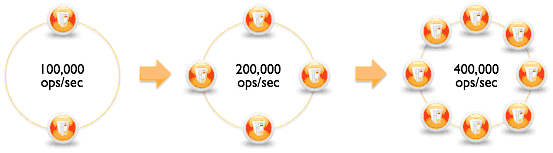
\includegraphics[width=\textwidth]{images/cassandra-linear-scalability.png}\hspace{10mm}  
%   \caption{The linear scalability from 100k to 400k requests per second}
%   \label{fig:archLinearScale}
% \end{figure}



\subsection{Cassandra Query Language}
\label{sec:theory:cassandra:cql}
Cassandra Query Language (CQL)\footnote{Cassandra from version 3.0 is released in a tick-tock manner, which means that there are frequent releases. CQL changes fast and gets new features almost every release} is the query language, similar in syntax to SQL, but provides only limited functionality compared to SQL, as there are no joins and inner queries. 

Cassandra provides CQL on top of logical data model, which introduces tables instead of column families and enforces table schema. Each row in a table has the same sequence of columns. Translation between physical and logical data models is done by means of key prefixes, so that all rows in a table $a$ have keys, which start with letter $a$. The same rule holds for columns; column names are embedded in keys.

CQL provides select, insert, update and delete statements. Select statement's \emph{where} clause supports equality condition on the partition key columns and restrictions such as: IN, =, >, >=, <= and < on the clustering columns. Columns, which are not part of the primary key cannot be restricted in the \emph{where} clause. Listing \ref{lst:cqlSelect} shows two examples of select statements, first with equality restriction on the partition key column \emph{user_id}, second with equality restrictions on the partition key columns: \emph{cluster}, \emph{date}, \emph{datacenter}, and range restrictions on the clustering key columns: \emph{hour} and \emph{minute}.
%Cassandra uses binary protocol named Cassandra Query Language (CQL). In order to do anything with database, we need to use a driver that speaks binary protocol. 

\begin{lstlisting}[style=outcode,label={lst:cqlSelect},caption={Examples of CQL select statements}]
SELECT user_name, user_email 
FROM app.users 
WHERE user_id=10123;
    
SELECT * FROM app.requests
WHERE cluster='cluster1'
AND date='2015/06/05'
AND datacenter='EU_NORTH'
AND (hour, minute)>=(12, 0) 
AND (hour, minute)<=(15, 30);
\end{lstlisting}


\subsection{Write path}
Cassandra write path \cite{CassandraWritePath} shown of Figure \ref{fig:writePath} consists of several stages. Writing starts with logging of a write in the \emph{commit log} so that writes are durable and survive permanently even if power fails on a node. 
Nextly, data is written to the \emph{memtable}, which is in-memory table that stores writes in sorted order.
If memtable exceeds its limit of memory then data from the memable are flushed to disk to files called \emph{SSTables}. SSTables are immutable after memtable is flushed. A single partition is typically stored across multiple SSTable files, thus read path has multiple files to read (more on read path in Section \ref{sec:readPath}).

When a new SSTable is created, Cassandra creates additional supporting files, which include: \begin{enumerate}
\item primary index -- index of the row keys with pointers to their positions in the data file,
\item bloom filter -- a structure stored in momery that checks if row data exists in the memtable before accessing SSTables on disk,
\item Compression information -- holds inforamtion about uncompressed data length and chunk offsets,
\item statistics -- statistical metadata about content in the SSTable,
\item digest -- file holding checksum of the data file,
\item crc -- file holding the CRC32 for data chunks,
\item summary -- a sample of the partition index stored in memory,
\item table of contents -- a file that stores the list of all components for the SSTable,
\item secondary index -- built-in secondary index.
\end{enumerate}

Over time Cassandra writes many timestamped versions of a row and many SSTables. This means that Cassandra must access more and more SSTables to retrieve an entire row of data. 
Compaction is a process of merging SSTables together so that old versions of rows are discarded preserving only most recent version. Compaction reduces disk usage by removing old data and improves read performance by limiting number of SSTables to read from.

\begin{figure}[H]
\centering
\begin{tikzpicture}[>=stealth',shorten >=1pt,auto,node distance=3.5cm,
  thick,
  node/.style={circle,fill=blue!20,draw,
  ,minimum size=5mm},
  main node 2/.style={circle,fill=blue!20,draw,
  ,minimum size=5mm},
  main node 3/.style={circle,dashed,fill=orange!60,draw,
  ,minimum size=5mm},
  main node 4/.style={circle,dashed,fill=red!20,draw,
  ,minimum size=5mm},
  database/.style={
      cylinder,
      cylinder uses custom fill,
      cylinder body fill=blue!20,
      cylinder end fill=blue!10,
      shape border rotate=90,
      aspect=0.25,
      draw
    }]

\node[node] (write) at (-4,8) {Write data};


\node[database,text height=1.5cm] (commitLog) at (0,0) {Commit log};

\draw[thick, dashed, line width=1mm, black] (-5,5) node[below] {Memory} node[above] {Disk} -- ++(15,0);


\node[draw=blue,line width=5mm, align=center,thick,text height=2cm, rounded corners=0.55cm, text width=3cm,inner sep=2pt] (memtable) at (4,8) {Memtable}; 

\draw[thick,black, ->] (write) -- (memtable);



\node[draw=blue,fill=blue!20,line width=5mm, align=center,thick,text height=3cm, rounded corners=0.55cm, text width=4cm,inner sep=2pt] (ssTable) at (4,0) {SSTable}; 

\draw[thick,dashed,black, ->] (memtable) -- ++(4,0) -- ++(0,-8) node[midway] {Flush} -- (ssTable);

\draw[thick,black,->] (0,8) -- (commitLog);

\end{tikzpicture}
\caption{Write path}
  \label{fig:writePath}
\end{figure}

\subsection{Read path}
\label{sec:readPath}
To read a partition, Cassandra has to combine data from the active memtable and potentially multiple SSTables \cite{CassandraReadPath}. Reading path is optimized in a way that reduces number of SSTables that need to be read. 

Figure \ref{fig:readPath} presents Cassandra's read path. There are several stages on the read path to find where the data is stored. Reading starts from reading the memtable followed by reading from row cache. It then checks bloom filters if SSTable might have the data. If bloom filter is positive then the SSTable might have the data, but does not have to. Cassandra goes directly to the compression offset map if a partition key is found in the partition key cache. Otherwise it checks partition summary followed by partition index and then goes to compression offset map, which allows to locate the data in the SSTable data file. At the end, Cassandra fetches the data from the SSTable on disk. The same process is performed for all SSTables, which have positive bloom filters, thus compaction and reducing number of SSTables is important for read performance.


\begin{figure}[H]
\centering
\begin{tikzpicture}[>=stealth',shorten >=1pt,auto,node distance=3.5cm,
  thick,
  node/.style={circle,fill=blue!20,draw,
  ,minimum size=5mm},
  bloomPositive/.style={circle,fill=blue!80,draw,
  ,minimum size=5mm},
  bloomNegative/.style={circle,fill=red!80,draw,
  ,minimum size=5mm},
  main node 4/.style={circle,dashed,fill=red!20,draw,
  ,minimum size=5mm},
  database/.style={
      cylinder,
      cylinder uses custom fill,
      cylinder body fill=blue!20,
      cylinder end fill=blue!10,
      shape border rotate=90,
      aspect=0.25,
      draw
    }]

\node[node] (read) at (-12,7) {Read data};

\node[draw=blue,line width=5mm, align=center,thick,text height=0.8cm, rounded corners=0.55cm, text width=3cm,inner sep=2pt] (bloomFilter) at (-5,7) {Bloom filter}; 

\node[draw=blue,line width=5mm, align=center,thick,text height=0.8cm, rounded corners=0.1cm, text width=3cm,inner sep=2pt] (partitionKeyCache) at (0,3) {Partition key cache};

\node[draw=blue,line width=5mm, rounded corners=0.1cm,align=center,thick,text height=0.8cm, text width=2cm,inner sep=2pt] (partitionSummary) at (-4,3) {Partition summary};

\node[draw=blue,line width=5mm, rounded corners=0.1cm,align=center,thick,text height=3cm, text width=0.5cm,inner sep=2pt] (compressionOffsets) at (-9,3) {Compression offsets};

\node[draw=blue,line width=5mm, rounded corners=0.1cm,align=center,thick,text height=2cm, text width=2cm,inner sep=2pt] (partitionIndex) at (-6,-4) {Partition index};

\node[draw=blue,line width=5mm, rounded corners=0.1cm,align=center,thick,text height=4cm, text width=2cm,inner sep=2pt] (data) at (-11,-4) {Data};

\draw[thick,black, ->] (read) -- (bloomFilter);

\draw[thick,black] (bloomFilter) -- ++(0,1) node[bloomPositive] {};
\draw[thick,black] (bloomFilter) -- ++(0,-1) node[bloomNegative] {};

\draw[thick, dashed, line width=1mm, black] (-12,0) node[below] {Memory} node[above] {Disk} -- ++(13,0);


\draw[thick,black, ->] (bloomFilter) -- ++(5,0) -- (partitionKeyCache);

\draw[thick,black, ->] (partitionKeyCache) -- (partitionSummary);

 \draw[thick,black, ->] (partitionKeyCache) -- ++(0,-9) -- ++(-9,0) -- (compressionOffsets);

 \draw[thick,black, ->] (partitionSummary) -- ++(0,-7) -- (partitionIndex);

\draw[thick,black, ->] (partitionIndex) -- ++(-2,0) -- ++(0,7) -- (compressionOffsets);

\draw[thick,black, ->] (compressionOffsets) -- ++(-2,0) -- (data);

\draw[thick,black, ->] (data) -- ++(-2,0) node[below] {Return row};

% \node[draw=blue,fill=blue!20,line width=5mm, align=center,thick,text height=3cm, rounded corners=0.55cm, text width=4cm,inner sep=2pt] (ssTable) at (4,0) {SSTable}; 

% \draw[thick,black,->] (0,8) -- (commitLog);

\end{tikzpicture}
\caption{Read path}
  \label{fig:readPath}
\end{figure}
 
\subsection{Use cases}
Cassandra is a general purpose non-relational database, however there are areas in which Cassandra excels over other databases:
\begin{itemize}
\item internet of things applications -- Cassandra is able to consume large quantity of incoming data\footnote{depends on cluster size} from devices, sensors and similar internet connected devices,
%\item E-commerce - durable shopping cart protection combined with fast product catalog browsing
%\item Messaging - Cassandra serves as the database for mobile phone applications
\item data analytics -- Apache Spark is an engine to perform large-scale data processing \cite{ApacheSpark} supports Cassandra, as one of its data sources.
Integration with Cassandra is token aware, thus it knows where data are on the cluster. Spark tries to load data locally if possible to avoid network overhead. Moreover it supports server-side filters that allow Cassandra to filter data before loading it in for analysis,
\item storage of time series data -- Cassandra's fast writes, wide-rows and ability to read only particular data ranges are well suited for time series based applications, because such data fits natively into the data model.
\end{itemize} 

\subsection{Transactions}
Cassandra provides \lwt, which are transactions limited to a single partition.
Comparison to the other distributed transaction implementations was provided in Section \ref{sec:theory:transactions:lwt}.

\subsubsection{Compared to RDBMS}
Figure \ref{fig:cassandraToRdbms} presents comparison of Cassandra and RDBMS.
\begin{figure}[H]
  %\centering
  \setlength{\unitlength}{1.3cm}  
  \subfloat{
    \renewcommand{\tabcolsep}{0.1cm}
    \resizebox{\textwidth}{!}{\begin{tabular}{c|c}
      \toprule
      RDBMS & Cassandra  \\ \midrule
      manages structured data      &  manages any type of data    \\
      ACID transactions 		   &  simple transactions supported by LWT \\
      SQL & CQL \\
      scales vertically & scales horizontally \\
      master-slave architecture & masterless, share nothing architecture \\
      %denormalization is the bad practice & denormalization is the best practice \\
      single points of failure with failover & no single points of failure \\  \bottomrule      
    \end{tabular}}
  }
  \caption{RDBMS compared to Cassandra}
  \label{fig:cassandraToRdbms}
\end{figure}

\subsection{Eventual consistency}\label{sec:theory:eventualConsistency}
In terms of CAP \cite{brewer2000towards} \cite{Brewer:2012ba} Cassandra is the \emph{AP} database with eventual consistency, which means that over time data becomes consistent on all nodes, but there are no guarantees about the time it takes. Cassandra uses techniques such as: \begin{enumerate*}[label=\alph*)]
\item \emph{hinted handoff} - stores a message for the currently unavailable replica about the modification and sends it to the replica when it comes back up \cite{CassandraHintedHandoff},  
\item \emph{read repairs} - detects inconsistency in data during read and repairs it by immediate updates \cite{CassandraReadRepair},  \end{enumerate*} to pro-actively reduce incosistency in data during normal operations.